\documentclass[a4paper,11pt]{article}
\usepackage[T1]{fontenc}
\usepackage[utf8]{inputenc}
\usepackage[english]{babel}
\usepackage{amsmath,amssymb,mathtools}
\usepackage[margin=2.2cm]{geometry}
\usepackage{tikz}
\usepackage[most]{tcolorbox}
\setlength{\parindent}{0pt}
\setlength{\parskip}{5pt}
\providecommand{\explainmode}{0}
\newif\ifexplain
\ifnum\explainmode=1 \explaintrue\fi
\newtcolorbox{erklbox}{colback=blue!4,colframe=blue!40,breakable,boxrule=.5pt,title=Erklärung}
\newcommand{\explain}[1]{\ifexplain\begin{erklbox}#1\end{erklbox}\fi}
\newcommand{\explainfig}[1]{\ifexplain\begin{center}#1\end{center}\fi}
\newcommand{\why}[1]{\text{\small #1}}
\newcommand{\angabe}[1]{\textit{#1}\par}
\newcommand{\aufgabe}[1]{\section*{Exercise #1}}
\newcommand{\teil}[1]{\subsection*{(#1)}}
\newcommand{\at}[1]{\texttt{#1}}
\begin{document}
\begin{center}{\Large Exercise sheet 1}\\Logic Programming (621.315), Winter semester 2026\\Raphael Bleier\\Demonstration: 21 October 2026\end{center}
\explain{Ein Atom ist hier eine einzelne Aussage, etwa $\at{bird(tweety)}$. Ein Modell erfüllt alle Regeln, muss aber nicht die kleinste begründbare Menge sein. Ein Answer Set ist die kleinste abgeschlossene Menge seines eigenen Redukts. Default-Negation \texttt{not a} prüft, ob $a$ im Kandidaten fehlt; sie ist keine zusätzliche Aussage $\neg a$. Wir verwenden die Begriffe und die Notation $\operatorname{Cn}(P)$ aus den Kursnotizen zu positiven und normalen Programmen.}
\section*{Quiz}
\paragraph{1}\angabe{Each positive logic program has at most one model.}
Take $P=\{a\mathbin{:-}b\}$. Both $\varnothing$ and $\{a,b\}$ satisfy the rule; they are distinct models. $\square$
\[
\boxed{\text{False}}
\]
\explain{Hier unterscheiden wir gewöhnliche Modelle von Answer Sets. Für ein Answer Set dürfen keine Atome ohne eine Herleitung aus dem Redukt übrig bleiben. Die Aussage über normale Programme nutzt ausdrücklich die Kursdefinition mit genau einem Atom im Regelkopf.}
\paragraph{2}\angabe{Each positive logic program has at most one answer set.}
A positive program has a unique least model, obtained by iterating its consequence operator. Its answer set is this least model. $\square$
\[
\boxed{\text{True}}
\]
\explain{Hier unterscheiden wir gewöhnliche Modelle von Answer Sets. Für ein Answer Set dürfen keine Atome ohne eine Herleitung aus dem Redukt übrig bleiben. Die Aussage über normale Programme nutzt ausdrücklich die Kursdefinition mit genau einem Atom im Regelkopf.}
\paragraph{3}\angabe{Each normal logic program has at least one model.}
Under the course definition, every rule has an atom in its head (no headless constraints). The interpretation $A(P)$ containing all atoms satisfies every rule, since every head is true. $\square$
\[
\boxed{\text{True}}
\]
\explain{Hier unterscheiden wir gewöhnliche Modelle von Answer Sets. Für ein Answer Set dürfen keine Atome ohne eine Herleitung aus dem Redukt übrig bleiben. Die Aussage über normale Programme nutzt ausdrücklich die Kursdefinition mit genau einem Atom im Regelkopf.}
\paragraph{4}\angabe{Each normal logic program has at least one answer set.}
Take $P=\{a\mathbin{:-}\mathop{not}a\}$. For $X=\varnothing$, the reduct contains the fact $a$ and has least model $\{a\}$. For $X=\{a\}$, the reduct is empty and has least model $\varnothing$. Neither candidate equals its reduct least model. $\square$
\[
\boxed{\text{False}}
\]
\explain{Hier unterscheiden wir gewöhnliche Modelle von Answer Sets. Für ein Answer Set dürfen keine Atome ohne eine Herleitung aus dem Redukt übrig bleiben. Die Aussage über normale Programme nutzt ausdrücklich die Kursdefinition mit genau einem Atom im Regelkopf.}
\aufgabe{1.1}
\angabe{Determine the answer set of the following positive logic programs.}
\teil{a}
Rule numbers refer to the following order (one rule ends at each period).
\begin{small}
\begin{verbatim}
a.
b :- e.
b :- f.
c :- b, f.
c :- d, g.
d.
e :- b, d.
g :- a, b.
g :- a, d.
\end{verbatim}
\end{small}
\explain{Das Programm enthält keine Default-Negation. Wir beginnen bei der leeren Menge und wenden nur Regeln an, deren Körper bereits erfüllt ist. Fakten starten die Herleitung. Eine positive Schleife ohne diesen Start liefert dagegen keine Atome.}
\[
M_0=\varnothing
\]
\begin{align*}
M_{1} &= M_{0}\cup \{\at{a}\} && \why{fact, rule 1}
\end{align*}
\explain{Diese Regel hat keinen Körper. Ihr Kopf $\at{a}$ ist damit ein Fakt und muss in die Menge.}
\begin{align*}
M_{2} &= M_{1}\cup \{\at{d}\} && \why{fact, rule 6}
\end{align*}
\explain{Diese Regel hat keinen Körper. Ihr Kopf $\at{d}$ ist damit ein Fakt und muss in die Menge.}
\begin{align*}
M_{3} &= M_{2}\cup \{\at{g}\} && \why{rule 9}
\end{align*}
\explain{Für $\at{g}$ brauchen wir $\at{a}$ und $\at{d}$. Weil diese Voraussetzungen bereits hergeleitet sind, dürfen wir den Regelkopf jetzt aufnehmen und alle bisherigen Atome behalten; bei einer fehlenden Voraussetzung würde diese Regel dagegen noch nichts beitragen.}
\begin{align*}
M_{4} &= M_{3}\cup \{\at{c}\} && \why{rule 5}
\end{align*}
\explain{Für $\at{c}$ brauchen wir $\at{d}$ und $\at{g}$. Weil diese Voraussetzungen bereits hergeleitet sind, dürfen wir den Regelkopf jetzt aufnehmen und alle bisherigen Atome behalten; bei einer fehlenden Voraussetzung würde diese Regel dagegen noch nichts beitragen.}
No rule has a true body and a head outside $M_{4}$; hence this is the least fixed point.
\[
\operatorname{Cn}(R)=\{\at{a},\;\at{c},\;\at{d},\;\at{g}\}
\]
Neither $b$ nor $e$ has an initial derivation; $f$ has no head rule. The rules linking $b,e$ cannot start.
\explainfig{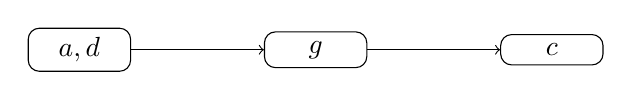
\begin{tikzpicture}[every node/.style={draw,rounded corners,minimum width=1.3cm}]\node (ad) at (0,0) {$a,d$};\node (g) at (3,0) {$g$};\node (c) at (6,0) {$c$};\draw[->] (ad)--(g);\draw[->] (g)--(c);\end{tikzpicture}}
\explain{Die Pfeile zeigen den Weg vom Faktpaar zur neuen Aussage. Für $g$ brauchen wir $a,d$; für $c$ danach noch $d$, das als Fakt bereits vorhanden ist. Der Kreis zwischen $b$ und $e$ liegt außerhalb dieses Herleitungswegs und bekommt keinen Start.}
\[
\boxed{X=\{\at{a},\;\at{c},\;\at{d},\;\at{g}\}}
\]
\explain{Die Probe besteht aus zwei Teilen: Jede aufgenommene Aussage hat oben eine passende Regel. Am Ende kann keine Regel ein weiteres Atom hinzufügen. Damit ist die Menge ein Modell und zugleich das kleinste Modell.}
\teil{b}
Rule numbers refer to the following order (one rule ends at each period).
\begin{small}
\begin{verbatim}
likes(kate,fish).
likes(kate,soup).
likes(mike,beef).
likes(mike,cake).
likes(paul,duck).
likes(paul,pork).
likes(tina,beef).
likes(tina,soup).
order(beef) :- likes(mike,beef), likes(tina,beef).
order(soup) :- likes(kate,soup), likes(tina,soup).
happy(kate) :- likes(kate,fish), order(fish).
happy(kate) :- likes(kate,soup), order(soup).
happy(mike) :- likes(mike,beef), order(beef).
happy(mike) :- likes(mike,cake), order(cake).
happy(paul) :- likes(paul,duck), order(duck).
happy(paul) :- likes(paul,pork), order(pork).
happy(tina) :- likes(tina,beef), order(beef).
happy(tina) :- likes(tina,soup), order(soup).
\end{verbatim}
\end{small}
\explain{Das Programm enthält keine Default-Negation. Wir beginnen bei der leeren Menge und wenden nur Regeln an, deren Körper bereits erfüllt ist. Fakten starten die Herleitung. Eine positive Schleife ohne diesen Start liefert dagegen keine Atome.}
\[
M_0=\varnothing
\]
\begin{align*}
M_{1} &= M_{0}\cup \{\at{likes(kate,fish)}\} && \why{fact, rule 1}
\end{align*}
\explain{Diese Regel hat keinen Körper. Ihr Kopf $\at{likes(kate,fish)}$ ist damit ein Fakt und muss in die Menge.}
\begin{align*}
M_{2} &= M_{1}\cup \{\at{likes(kate,soup)}\} && \why{fact, rule 2}
\end{align*}
\explain{Diese Regel hat keinen Körper. Ihr Kopf $\at{likes(kate,soup)}$ ist damit ein Fakt und muss in die Menge.}
\begin{align*}
M_{3} &= M_{2}\cup \{\at{likes(mike,beef)}\} && \why{fact, rule 3}
\end{align*}
\explain{Diese Regel hat keinen Körper. Ihr Kopf $\at{likes(mike,beef)}$ ist damit ein Fakt und muss in die Menge.}
\begin{align*}
M_{4} &= M_{3}\cup \{\at{likes(mike,cake)}\} && \why{fact, rule 4}
\end{align*}
\explain{Diese Regel hat keinen Körper. Ihr Kopf $\at{likes(mike,cake)}$ ist damit ein Fakt und muss in die Menge.}
\begin{align*}
M_{5} &= M_{4}\cup \{\at{likes(paul,duck)}\} && \why{fact, rule 5}
\end{align*}
\explain{Diese Regel hat keinen Körper. Ihr Kopf $\at{likes(paul,duck)}$ ist damit ein Fakt und muss in die Menge.}
\begin{align*}
M_{6} &= M_{5}\cup \{\at{likes(paul,pork)}\} && \why{fact, rule 6}
\end{align*}
\explain{Diese Regel hat keinen Körper. Ihr Kopf $\at{likes(paul,pork)}$ ist damit ein Fakt und muss in die Menge.}
\begin{align*}
M_{7} &= M_{6}\cup \{\at{likes(tina,beef)}\} && \why{fact, rule 7}
\end{align*}
\explain{Diese Regel hat keinen Körper. Ihr Kopf $\at{likes(tina,beef)}$ ist damit ein Fakt und muss in die Menge.}
\begin{align*}
M_{8} &= M_{7}\cup \{\at{likes(tina,soup)}\} && \why{fact, rule 8}
\end{align*}
\explain{Diese Regel hat keinen Körper. Ihr Kopf $\at{likes(tina,soup)}$ ist damit ein Fakt und muss in die Menge.}
\begin{align*}
M_{9} &= M_{8}\cup \{\at{order(beef)}\} && \why{rule 9}
\end{align*}
\explain{Für $\at{order(beef)}$ brauchen wir $\at{likes(mike,beef)}$ und $\at{likes(tina,beef)}$. Weil diese Voraussetzungen bereits hergeleitet sind, dürfen wir den Regelkopf jetzt aufnehmen und alle bisherigen Atome behalten; bei einer fehlenden Voraussetzung würde diese Regel dagegen noch nichts beitragen.}
\begin{align*}
M_{10} &= M_{9}\cup \{\at{order(soup)}\} && \why{rule 10}
\end{align*}
\explain{Für $\at{order(soup)}$ brauchen wir $\at{likes(kate,soup)}$ und $\at{likes(tina,soup)}$. Weil diese Voraussetzungen bereits hergeleitet sind, dürfen wir den Regelkopf jetzt aufnehmen und alle bisherigen Atome behalten; bei einer fehlenden Voraussetzung würde diese Regel dagegen noch nichts beitragen.}
\begin{align*}
M_{11} &= M_{10}\cup \{\at{happy(kate)}\} && \why{rule 12}
\end{align*}
\explain{Für $\at{happy(kate)}$ brauchen wir $\at{likes(kate,soup)}$ und $\at{order(soup)}$. Weil diese Voraussetzungen bereits hergeleitet sind, dürfen wir den Regelkopf jetzt aufnehmen und alle bisherigen Atome behalten; bei einer fehlenden Voraussetzung würde diese Regel dagegen noch nichts beitragen.}
\begin{align*}
M_{12} &= M_{11}\cup \{\at{happy(mike)}\} && \why{rule 13}
\end{align*}
\explain{Für $\at{happy(mike)}$ brauchen wir $\at{likes(mike,beef)}$ und $\at{order(beef)}$. Weil diese Voraussetzungen bereits hergeleitet sind, dürfen wir den Regelkopf jetzt aufnehmen und alle bisherigen Atome behalten; bei einer fehlenden Voraussetzung würde diese Regel dagegen noch nichts beitragen.}
\begin{align*}
M_{13} &= M_{12}\cup \{\at{happy(tina)}\} && \why{rule 17}
\end{align*}
\explain{Für $\at{happy(tina)}$ brauchen wir $\at{likes(tina,beef)}$ und $\at{order(beef)}$. Weil diese Voraussetzungen bereits hergeleitet sind, dürfen wir den Regelkopf jetzt aufnehmen und alle bisherigen Atome behalten; bei einer fehlenden Voraussetzung würde diese Regel dagegen noch nichts beitragen.}
No rule has a true body and a head outside $M_{13}$; hence this is the least fixed point.
\[
\operatorname{Cn}(R)=\left\{\begin{gathered}\at{happy(kate)},\;\at{happy(mike)},\;\at{happy(tina)},\\\at{likes(kate,fish)},\;\at{likes(kate,soup)},\\\at{likes(mike,beef)},\;\at{likes(mike,cake)},\\\at{likes(paul,duck)},\;\at{likes(paul,pork)},\\\at{likes(tina,beef)},\;\at{likes(tina,soup)},\;\at{order(beef)},\\\at{order(soup)}\end{gathered}\right\}
\]
\[
\boxed{X=\left\{\begin{gathered}\at{happy(kate)},\;\at{happy(mike)},\;\at{happy(tina)},\\\at{likes(kate,fish)},\;\at{likes(kate,soup)},\\\at{likes(mike,beef)},\;\at{likes(mike,cake)},\\\at{likes(paul,duck)},\;\at{likes(paul,pork)},\\\at{likes(tina,beef)},\;\at{likes(tina,soup)},\;\at{order(beef)},\\\at{order(soup)}\end{gathered}\right\}}
\]
\explain{Die Probe besteht aus zwei Teilen: Jede aufgenommene Aussage hat oben eine passende Regel. Am Ende kann keine Regel ein weiteres Atom hinzufügen. Damit ist die Menge ein Modell und zugleich das kleinste Modell.}
\aufgabe{1.2}
\angabe{Determine the reducts for the given candidate sets and decide which candidates are answer sets.}
\teil{a}
Rule numbers refer to the following order (one rule ends at each period).
\begin{small}
\begin{verbatim}
a :- b.
b :- not c.
c :- not b.
d :- a, e.
e.
\end{verbatim}
\end{small}
\paragraph{Candidate $X_1$}
\[
X=\{\at{a},\;\at{b},\;\at{d},\;\at{e}\}
\]
Reduct $R=P^X$: delete a rule if a default-negated atom belongs to $X$; remove the remaining default negations. Deletion decisions use the order in $P$; the subsequent derivation uses the order in the displayed reduct $R$.
Rule 2 is retained because $\{\at{c}\}\cap X=\varnothing$; its default negations are removed.

Rule 3 is deleted because $\{\at{b}\}\subseteq X$.

Rule numbers refer to the following order (one rule ends at each period).
\begin{small}
\begin{verbatim}
a :- b.
b.
d :- a, e.
e.
\end{verbatim}
\end{small}
\explain{Beim Redukt bleibt die Kandidatenmenge fest. Wir entscheiden zuerst, welche Regeln wegfallen. Erst danach berechnen wir aus den verbleibenden positiven Regeln die kleinste abgeschlossene Menge. Ein Modell allein reicht nicht: Diese Menge muss genau der Kandidat sein.}
\[
M_0=\varnothing
\]
\begin{align*}
M_{1} &= M_{0}\cup \{\at{b}\} && \why{fact, rule 2}
\end{align*}
\explain{Diese Regel hat keinen Körper. Ihr Kopf $\at{b}$ ist damit ein Fakt und muss in die Menge.}
\begin{align*}
M_{2} &= M_{1}\cup \{\at{e}\} && \why{fact, rule 4}
\end{align*}
\explain{Diese Regel hat keinen Körper. Ihr Kopf $\at{e}$ ist damit ein Fakt und muss in die Menge.}
\begin{align*}
M_{3} &= M_{2}\cup \{\at{a}\} && \why{rule 1}
\end{align*}
\explain{Für $\at{a}$ brauchen wir $\at{b}$. Weil diese Voraussetzungen bereits hergeleitet sind, dürfen wir den Regelkopf jetzt aufnehmen und alle bisherigen Atome behalten; bei einer fehlenden Voraussetzung würde diese Regel dagegen noch nichts beitragen.}
\begin{align*}
M_{4} &= M_{3}\cup \{\at{d}\} && \why{rule 3}
\end{align*}
\explain{Für $\at{d}$ brauchen wir $\at{a}$ und $\at{e}$. Weil diese Voraussetzungen bereits hergeleitet sind, dürfen wir den Regelkopf jetzt aufnehmen und alle bisherigen Atome behalten; bei einer fehlenden Voraussetzung würde diese Regel dagegen noch nichts beitragen.}
No rule has a true body and a head outside $M_{4}$; hence this is the least fixed point.
\[
\operatorname{Cn}(R)=\{\at{a},\;\at{b},\;\at{d},\;\at{e}\}
\]
\[
\operatorname{Cn}(P^X)=X
\]
\[
\boxed{X\text{ is an answer set.}}
\]
\paragraph{Candidate $X_2$}
\[
X=\{\at{b},\;\at{e}\}
\]
Reduct $R=P^X$: delete a rule if a default-negated atom belongs to $X$; remove the remaining default negations. Deletion decisions use the order in $P$; the subsequent derivation uses the order in the displayed reduct $R$.
Rule 2 is retained because $\{\at{c}\}\cap X=\varnothing$; its default negations are removed.

Rule 3 is deleted because $\{\at{b}\}\subseteq X$.

Rule numbers refer to the following order (one rule ends at each period).
\begin{small}
\begin{verbatim}
a :- b.
b.
d :- a, e.
e.
\end{verbatim}
\end{small}
\explain{Beim Redukt bleibt die Kandidatenmenge fest. Wir entscheiden zuerst, welche Regeln wegfallen. Erst danach berechnen wir aus den verbleibenden positiven Regeln die kleinste abgeschlossene Menge. Ein Modell allein reicht nicht: Diese Menge muss genau der Kandidat sein.}
\[
M_0=\varnothing
\]
\begin{align*}
M_{1} &= M_{0}\cup \{\at{b}\} && \why{fact, rule 2}
\end{align*}
\explain{Diese Regel hat keinen Körper. Ihr Kopf $\at{b}$ ist damit ein Fakt und muss in die Menge.}
\begin{align*}
M_{2} &= M_{1}\cup \{\at{e}\} && \why{fact, rule 4}
\end{align*}
\explain{Diese Regel hat keinen Körper. Ihr Kopf $\at{e}$ ist damit ein Fakt und muss in die Menge.}
\begin{align*}
M_{3} &= M_{2}\cup \{\at{a}\} && \why{rule 1}
\end{align*}
\explain{Für $\at{a}$ brauchen wir $\at{b}$. Weil diese Voraussetzungen bereits hergeleitet sind, dürfen wir den Regelkopf jetzt aufnehmen und alle bisherigen Atome behalten; bei einer fehlenden Voraussetzung würde diese Regel dagegen noch nichts beitragen.}
\begin{align*}
M_{4} &= M_{3}\cup \{\at{d}\} && \why{rule 3}
\end{align*}
\explain{Für $\at{d}$ brauchen wir $\at{a}$ und $\at{e}$. Weil diese Voraussetzungen bereits hergeleitet sind, dürfen wir den Regelkopf jetzt aufnehmen und alle bisherigen Atome behalten; bei einer fehlenden Voraussetzung würde diese Regel dagegen noch nichts beitragen.}
No rule has a true body and a head outside $M_{4}$; hence this is the least fixed point.
\[
\operatorname{Cn}(R)=\{\at{a},\;\at{b},\;\at{d},\;\at{e}\}
\]
\[
\operatorname{Cn}(P^X)\ne X
\]
\[
\boxed{X\text{ is not an answer set.}}
\]
Missing from the candidate: $\{\at{a},\;\at{d}\}$.
\teil{b}
Rule numbers refer to the following order (one rule ends at each period).
\begin{small}
\begin{verbatim}
a :- not b.
a :- d.
b :- not c.
c :- a, not b.
d :- a.
d :- not c, not e.
e :- b, not a.
e :- d.
\end{verbatim}
\end{small}
\paragraph{Candidate $X_1$}
\[
X=\{\at{a},\;\at{b},\;\at{d},\;\at{e}\}
\]
Reduct $R=P^X$: delete a rule if a default-negated atom belongs to $X$; remove the remaining default negations. Deletion decisions use the order in $P$; the subsequent derivation uses the order in the displayed reduct $R$.
Rule 1 is deleted because $\{\at{b}\}\subseteq X$.

Rule 3 is retained because $\{\at{c}\}\cap X=\varnothing$; its default negations are removed.

Rule 4 is deleted because $\{\at{b}\}\subseteq X$.

Rule 6 is deleted because $\{\at{e}\}\subseteq X$.

Rule 7 is deleted because $\{\at{a}\}\subseteq X$.

Rule numbers refer to the following order (one rule ends at each period).
\begin{small}
\begin{verbatim}
a :- d.
b.
d :- a.
e :- d.
\end{verbatim}
\end{small}
\explain{Beim Redukt bleibt die Kandidatenmenge fest. Wir entscheiden zuerst, welche Regeln wegfallen. Erst danach berechnen wir aus den verbleibenden positiven Regeln die kleinste abgeschlossene Menge. Ein Modell allein reicht nicht: Diese Menge muss genau der Kandidat sein.}
\[
M_0=\varnothing
\]
\begin{align*}
M_{1} &= M_{0}\cup \{\at{b}\} && \why{fact, rule 2}
\end{align*}
\explain{Diese Regel hat keinen Körper. Ihr Kopf $\at{b}$ ist damit ein Fakt und muss in die Menge.}
No rule has a true body and a head outside $M_{1}$; hence this is the least fixed point.
\[
\operatorname{Cn}(R)=\{\at{b}\}
\]
\[
\operatorname{Cn}(P^X)\ne X
\]
\[
\boxed{X\text{ is not an answer set.}}
\]
Unsupported candidate atoms: $\{\at{a},\;\at{d},\;\at{e}\}$.
\paragraph{Candidate $X_2$}
\[
X=\{\at{b},\;\at{e}\}
\]
Reduct $R=P^X$: delete a rule if a default-negated atom belongs to $X$; remove the remaining default negations. Deletion decisions use the order in $P$; the subsequent derivation uses the order in the displayed reduct $R$.
Rule 1 is deleted because $\{\at{b}\}\subseteq X$.

Rule 3 is retained because $\{\at{c}\}\cap X=\varnothing$; its default negations are removed.

Rule 4 is deleted because $\{\at{b}\}\subseteq X$.

Rule 6 is deleted because $\{\at{e}\}\subseteq X$.

Rule 7 is retained because $\{\at{a}\}\cap X=\varnothing$; its default negations are removed.

Rule numbers refer to the following order (one rule ends at each period).
\begin{small}
\begin{verbatim}
a :- d.
b.
d :- a.
e :- b.
e :- d.
\end{verbatim}
\end{small}
\explain{Beim Redukt bleibt die Kandidatenmenge fest. Wir entscheiden zuerst, welche Regeln wegfallen. Erst danach berechnen wir aus den verbleibenden positiven Regeln die kleinste abgeschlossene Menge. Ein Modell allein reicht nicht: Diese Menge muss genau der Kandidat sein.}
\[
M_0=\varnothing
\]
\begin{align*}
M_{1} &= M_{0}\cup \{\at{b}\} && \why{fact, rule 2}
\end{align*}
\explain{Diese Regel hat keinen Körper. Ihr Kopf $\at{b}$ ist damit ein Fakt und muss in die Menge.}
\begin{align*}
M_{2} &= M_{1}\cup \{\at{e}\} && \why{rule 4}
\end{align*}
\explain{Für $\at{e}$ brauchen wir $\at{b}$. Weil diese Voraussetzungen bereits hergeleitet sind, dürfen wir den Regelkopf jetzt aufnehmen und alle bisherigen Atome behalten; bei einer fehlenden Voraussetzung würde diese Regel dagegen noch nichts beitragen.}
No rule has a true body and a head outside $M_{2}$; hence this is the least fixed point.
\[
\operatorname{Cn}(R)=\{\at{b},\;\at{e}\}
\]
\[
\operatorname{Cn}(P^X)=X
\]
\[
\boxed{X\text{ is an answer set.}}
\]
\aufgabe{1.3}
\angabe{Find all answer sets of both programs from Exercise 1.2 without testing all interpretations.}
\teil{a}
The fact forces $e$. If $b\in X$, the rule for $c$ is deleted, so $c$ has no supporting rule. Thus $c\notin X$. The reduct contains the fact $b$; $a$ follows from $b$, and $d$ follows from $a,e$. This gives $X=\{a,b,d,e\}$. If $b\notin X$, the reduct contains the fact $c$. The rule for $b$ is then deleted. Neither $a$ nor $d$ can be derived, giving $X=\{c,e\}$. These two cases exhaust membership of $b$. $\square$
\explain{Wir teilen nur nach Atomen auf, die eine echte Entscheidung durch Default-Negation auslösen. Danach erzwingen Fakten und Regeln den Rest. Ein positiver Kreis begründet sich nicht selbst: Ohne Startregel bleibt er beim Aufbau der kleinsten Menge leer.}
\[
\boxed{\#\operatorname{AS}(P)=2}
\]
\paragraph{Answer set 1 and reduct check}
\[
X=\{\at{a},\;\at{b},\;\at{d},\;\at{e}\}
\]
Reduct $R=P^X$: delete a rule if a default-negated atom belongs to $X$; remove the remaining default negations. Deletion decisions use the order in $P$; the subsequent derivation uses the order in the displayed reduct $R$.
Rule 2 is retained because $\{\at{c}\}\cap X=\varnothing$; its default negations are removed.

Rule 3 is deleted because $\{\at{b}\}\subseteq X$.

Rule numbers refer to the following order (one rule ends at each period).
\begin{small}
\begin{verbatim}
a :- b.
b.
d :- a, e.
e.
\end{verbatim}
\end{small}
\explain{Beim Redukt bleibt die Kandidatenmenge fest. Wir entscheiden zuerst, welche Regeln wegfallen. Erst danach berechnen wir aus den verbleibenden positiven Regeln die kleinste abgeschlossene Menge. Ein Modell allein reicht nicht: Diese Menge muss genau der Kandidat sein.}
\[
M_0=\varnothing
\]
\begin{align*}
M_{1} &= M_{0}\cup \{\at{b}\} && \why{fact, rule 2}
\end{align*}
\explain{Diese Regel hat keinen Körper. Ihr Kopf $\at{b}$ ist damit ein Fakt und muss in die Menge.}
\begin{align*}
M_{2} &= M_{1}\cup \{\at{e}\} && \why{fact, rule 4}
\end{align*}
\explain{Diese Regel hat keinen Körper. Ihr Kopf $\at{e}$ ist damit ein Fakt und muss in die Menge.}
\begin{align*}
M_{3} &= M_{2}\cup \{\at{a}\} && \why{rule 1}
\end{align*}
\explain{Für $\at{a}$ brauchen wir $\at{b}$. Weil diese Voraussetzungen bereits hergeleitet sind, dürfen wir den Regelkopf jetzt aufnehmen und alle bisherigen Atome behalten; bei einer fehlenden Voraussetzung würde diese Regel dagegen noch nichts beitragen.}
\begin{align*}
M_{4} &= M_{3}\cup \{\at{d}\} && \why{rule 3}
\end{align*}
\explain{Für $\at{d}$ brauchen wir $\at{a}$ und $\at{e}$. Weil diese Voraussetzungen bereits hergeleitet sind, dürfen wir den Regelkopf jetzt aufnehmen und alle bisherigen Atome behalten; bei einer fehlenden Voraussetzung würde diese Regel dagegen noch nichts beitragen.}
No rule has a true body and a head outside $M_{4}$; hence this is the least fixed point.
\[
\operatorname{Cn}(R)=\{\at{a},\;\at{b},\;\at{d},\;\at{e}\}
\]
\[
\operatorname{Cn}(P^X)=X
\]
\[
\boxed{X\text{ is an answer set.}}
\]
\paragraph{Answer set 2 and reduct check}
\[
X=\{\at{c},\;\at{e}\}
\]
Reduct $R=P^X$: delete a rule if a default-negated atom belongs to $X$; remove the remaining default negations. Deletion decisions use the order in $P$; the subsequent derivation uses the order in the displayed reduct $R$.
Rule 2 is deleted because $\{\at{c}\}\subseteq X$.

Rule 3 is retained because $\{\at{b}\}\cap X=\varnothing$; its default negations are removed.

Rule numbers refer to the following order (one rule ends at each period).
\begin{small}
\begin{verbatim}
a :- b.
c.
d :- a, e.
e.
\end{verbatim}
\end{small}
\explain{Beim Redukt bleibt die Kandidatenmenge fest. Wir entscheiden zuerst, welche Regeln wegfallen. Erst danach berechnen wir aus den verbleibenden positiven Regeln die kleinste abgeschlossene Menge. Ein Modell allein reicht nicht: Diese Menge muss genau der Kandidat sein.}
\[
M_0=\varnothing
\]
\begin{align*}
M_{1} &= M_{0}\cup \{\at{c}\} && \why{fact, rule 2}
\end{align*}
\explain{Diese Regel hat keinen Körper. Ihr Kopf $\at{c}$ ist damit ein Fakt und muss in die Menge.}
\begin{align*}
M_{2} &= M_{1}\cup \{\at{e}\} && \why{fact, rule 4}
\end{align*}
\explain{Diese Regel hat keinen Körper. Ihr Kopf $\at{e}$ ist damit ein Fakt und muss in die Menge.}
No rule has a true body and a head outside $M_{2}$; hence this is the least fixed point.
\[
\operatorname{Cn}(R)=\{\at{c},\;\at{e}\}
\]
\[
\operatorname{Cn}(P^X)=X
\]
\[
\boxed{X\text{ is an answer set.}}
\]
The complete list of answer sets is:
\[
\boxed{X_1=\{\at{a},\;\at{b},\;\at{d},\;\at{e}\}}
\]
\[
\boxed{X_2=\{\at{c},\;\at{e}\}}
\]
\teil{b}
If $b\notin X$, the reduct contains the fact $a$. The rules for $d$, $e$, and $c$ then derive these three atoms. Since $c\in X$, the rule for $b$ is deleted. The only candidate in this case is $\{a,c,d,e\}$.

If $b\in X$, support for $b$ requires $c\notin X$. Also $e\in X$: if $a\in X$, the rules $d$ from $a$ and $e$ from $d$ force $e$; if $a\notin X$, the rule $e$ from $b,\mathop{not}a$ forces $e$. Therefore the rule with body $\mathop{not}c,\mathop{not}e$ is deleted. The remaining rules for $a,d$ form only the positive cycle $a$ from $d$, $d$ from $a$, which has no initial fact. Neither atom belongs to the least model. We obtain $\{b,e\}$. These two cases exhaust membership of $b$. $\square$
\explain{Wir teilen nur nach Atomen auf, die eine echte Entscheidung durch Default-Negation auslösen. Danach erzwingen Fakten und Regeln den Rest. Ein positiver Kreis begründet sich nicht selbst: Ohne Startregel bleibt er beim Aufbau der kleinsten Menge leer.}
\[
\boxed{\#\operatorname{AS}(P)=2}
\]
\paragraph{Answer set 1 and reduct check}
\[
X=\{\at{a},\;\at{c},\;\at{d},\;\at{e}\}
\]
Reduct $R=P^X$: delete a rule if a default-negated atom belongs to $X$; remove the remaining default negations. Deletion decisions use the order in $P$; the subsequent derivation uses the order in the displayed reduct $R$.
Rule 1 is retained because $\{\at{b}\}\cap X=\varnothing$; its default negations are removed.

Rule 3 is deleted because $\{\at{c}\}\subseteq X$.

Rule 4 is retained because $\{\at{b}\}\cap X=\varnothing$; its default negations are removed.

Rule 6 is deleted because $\{\at{c},\;\at{e}\}\subseteq X$.

Rule 7 is deleted because $\{\at{a}\}\subseteq X$.

Rule numbers refer to the following order (one rule ends at each period).
\begin{small}
\begin{verbatim}
a.
a :- d.
c :- a.
d :- a.
e :- d.
\end{verbatim}
\end{small}
\explain{Beim Redukt bleibt die Kandidatenmenge fest. Wir entscheiden zuerst, welche Regeln wegfallen. Erst danach berechnen wir aus den verbleibenden positiven Regeln die kleinste abgeschlossene Menge. Ein Modell allein reicht nicht: Diese Menge muss genau der Kandidat sein.}
\[
M_0=\varnothing
\]
\begin{align*}
M_{1} &= M_{0}\cup \{\at{a}\} && \why{fact, rule 1}
\end{align*}
\explain{Diese Regel hat keinen Körper. Ihr Kopf $\at{a}$ ist damit ein Fakt und muss in die Menge.}
\begin{align*}
M_{2} &= M_{1}\cup \{\at{c}\} && \why{rule 3}
\end{align*}
\explain{Für $\at{c}$ brauchen wir $\at{a}$. Weil diese Voraussetzungen bereits hergeleitet sind, dürfen wir den Regelkopf jetzt aufnehmen und alle bisherigen Atome behalten; bei einer fehlenden Voraussetzung würde diese Regel dagegen noch nichts beitragen.}
\begin{align*}
M_{3} &= M_{2}\cup \{\at{d}\} && \why{rule 4}
\end{align*}
\explain{Für $\at{d}$ brauchen wir $\at{a}$. Weil diese Voraussetzungen bereits hergeleitet sind, dürfen wir den Regelkopf jetzt aufnehmen und alle bisherigen Atome behalten; bei einer fehlenden Voraussetzung würde diese Regel dagegen noch nichts beitragen.}
\begin{align*}
M_{4} &= M_{3}\cup \{\at{e}\} && \why{rule 5}
\end{align*}
\explain{Für $\at{e}$ brauchen wir $\at{d}$. Weil diese Voraussetzungen bereits hergeleitet sind, dürfen wir den Regelkopf jetzt aufnehmen und alle bisherigen Atome behalten; bei einer fehlenden Voraussetzung würde diese Regel dagegen noch nichts beitragen.}
No rule has a true body and a head outside $M_{4}$; hence this is the least fixed point.
\[
\operatorname{Cn}(R)=\{\at{a},\;\at{c},\;\at{d},\;\at{e}\}
\]
\[
\operatorname{Cn}(P^X)=X
\]
\[
\boxed{X\text{ is an answer set.}}
\]
\paragraph{Answer set 2 and reduct check}
\[
X=\{\at{b},\;\at{e}\}
\]
Reduct $R=P^X$: delete a rule if a default-negated atom belongs to $X$; remove the remaining default negations. Deletion decisions use the order in $P$; the subsequent derivation uses the order in the displayed reduct $R$.
Rule 1 is deleted because $\{\at{b}\}\subseteq X$.

Rule 3 is retained because $\{\at{c}\}\cap X=\varnothing$; its default negations are removed.

Rule 4 is deleted because $\{\at{b}\}\subseteq X$.

Rule 6 is deleted because $\{\at{e}\}\subseteq X$.

Rule 7 is retained because $\{\at{a}\}\cap X=\varnothing$; its default negations are removed.

Rule numbers refer to the following order (one rule ends at each period).
\begin{small}
\begin{verbatim}
a :- d.
b.
d :- a.
e :- b.
e :- d.
\end{verbatim}
\end{small}
\explain{Beim Redukt bleibt die Kandidatenmenge fest. Wir entscheiden zuerst, welche Regeln wegfallen. Erst danach berechnen wir aus den verbleibenden positiven Regeln die kleinste abgeschlossene Menge. Ein Modell allein reicht nicht: Diese Menge muss genau der Kandidat sein.}
\[
M_0=\varnothing
\]
\begin{align*}
M_{1} &= M_{0}\cup \{\at{b}\} && \why{fact, rule 2}
\end{align*}
\explain{Diese Regel hat keinen Körper. Ihr Kopf $\at{b}$ ist damit ein Fakt und muss in die Menge.}
\begin{align*}
M_{2} &= M_{1}\cup \{\at{e}\} && \why{rule 4}
\end{align*}
\explain{Für $\at{e}$ brauchen wir $\at{b}$. Weil diese Voraussetzungen bereits hergeleitet sind, dürfen wir den Regelkopf jetzt aufnehmen und alle bisherigen Atome behalten; bei einer fehlenden Voraussetzung würde diese Regel dagegen noch nichts beitragen.}
No rule has a true body and a head outside $M_{2}$; hence this is the least fixed point.
\[
\operatorname{Cn}(R)=\{\at{b},\;\at{e}\}
\]
\[
\operatorname{Cn}(P^X)=X
\]
\[
\boxed{X\text{ is an answer set.}}
\]
The complete list of answer sets is:
\[
\boxed{X_1=\{\at{a},\;\at{c},\;\at{d},\;\at{e}\}}
\]
\[
\boxed{X_2=\{\at{b},\;\at{e}\}}
\]
\aufgabe{1.4}
\angabe{Determine all answer sets of the following normal logic programs.}
\teil{a}
Rule numbers refer to the following order (one rule ends at each period).
\begin{small}
\begin{verbatim}
canary(tweety).
penguin(tux).
bird(tweety) :- canary(tweety).
bird(tux) :- penguin(tux).
injured(tweety) :- bird(tweety), not ok(tweety).
ok(tweety) :- bird(tweety), not injured(tweety).
injured(tux) :- bird(tux), not ok(tux).
ok(tux) :- bird(tux), not injured(tux).
flies(tweety) :- ok(tweety), not penguin(tweety).
flies(tux) :- ok(tux), not penguin(tux).
\end{verbatim}
\end{small}
Both bird atoms follow from the facts. For each bird, at least one of $\at{injured}$ and $\at{ok}$ must hold: if neither held, the reduct would derive both from the bird atom. They cannot both hold, because then both supporting rules would be deleted. Thus each bird has exactly one of these two properties. The choices are independent. Tweety flies precisely when $\at{ok(tweety)}$ is chosen, since $\at{penguin(tweety)}$ has no supporting rule. The rule for Tux flying is always deleted by the penguin fact. The four combinations below exhaust the two independent binary choices. $\square$
\explain{Zuerst klären wir, welche Kombinationen überhaupt möglich sind. Gegenseitige Default-Negation lässt genau eine der beiden Eigenschaften zu. Eine Regel mit \texttt{not p} und Kopf $p$ kann einen Fall ausschließen, statt einfach $p$ zu einer stabilen Lösung hinzuzufügen. Die Redukt-Proben darunter prüfen jede verbliebene Kombination einzeln.}
\[
\boxed{\#\operatorname{AS}(P)=4}
\]
\paragraph{Answer set 1 and reduct check}
\[
X=\left\{\begin{gathered}\at{bird(tux)},\;\at{bird(tweety)},\;\at{canary(tweety)},\\\at{flies(tweety)},\;\at{injured(tux)},\;\at{ok(tweety)},\\\at{penguin(tux)}\end{gathered}\right\}
\]
Reduct $R=P^X$: delete a rule if a default-negated atom belongs to $X$; remove the remaining default negations. Deletion decisions use the order in $P$; the subsequent derivation uses the order in the displayed reduct $R$.
Rule 5 is deleted because $\{\at{ok(tweety)}\}\subseteq X$.

Rule 6 is retained because $\{\at{injured(tweety)}\}\cap X=\varnothing$; its default negations are removed.

Rule 7 is retained because $\{\at{ok(tux)}\}\cap X=\varnothing$; its default negations are removed.

Rule 8 is deleted because $\{\at{injured(tux)}\}\subseteq X$.

Rule 9 is retained because $\{\at{penguin(tweety)}\}\cap X=\varnothing$; its default negations are removed.

Rule 10 is deleted because $\{\at{penguin(tux)}\}\subseteq X$.

Rule numbers refer to the following order (one rule ends at each period).
\begin{small}
\begin{verbatim}
canary(tweety).
penguin(tux).
bird(tweety) :- canary(tweety).
bird(tux) :- penguin(tux).
ok(tweety) :- bird(tweety).
injured(tux) :- bird(tux).
flies(tweety) :- ok(tweety).
\end{verbatim}
\end{small}
\explain{Beim Redukt bleibt die Kandidatenmenge fest. Wir entscheiden zuerst, welche Regeln wegfallen. Erst danach berechnen wir aus den verbleibenden positiven Regeln die kleinste abgeschlossene Menge. Ein Modell allein reicht nicht: Diese Menge muss genau der Kandidat sein.}
\[
M_0=\varnothing
\]
\begin{align*}
M_{1} &= M_{0}\cup \{\at{canary(tweety)}\} && \why{fact, rule 1}
\end{align*}
\explain{Diese Regel hat keinen Körper. Ihr Kopf $\at{canary(tweety)}$ ist damit ein Fakt und muss in die Menge.}
\begin{align*}
M_{2} &= M_{1}\cup \{\at{penguin(tux)}\} && \why{fact, rule 2}
\end{align*}
\explain{Diese Regel hat keinen Körper. Ihr Kopf $\at{penguin(tux)}$ ist damit ein Fakt und muss in die Menge.}
\begin{align*}
M_{3} &= M_{2}\cup \{\at{bird(tux)}\} && \why{rule 4}
\end{align*}
\explain{Für $\at{bird(tux)}$ brauchen wir $\at{penguin(tux)}$. Weil diese Voraussetzungen bereits hergeleitet sind, dürfen wir den Regelkopf jetzt aufnehmen und alle bisherigen Atome behalten; bei einer fehlenden Voraussetzung würde diese Regel dagegen noch nichts beitragen.}
\begin{align*}
M_{4} &= M_{3}\cup \{\at{bird(tweety)}\} && \why{rule 3}
\end{align*}
\explain{Für $\at{bird(tweety)}$ brauchen wir $\at{canary(tweety)}$. Weil diese Voraussetzungen bereits hergeleitet sind, dürfen wir den Regelkopf jetzt aufnehmen und alle bisherigen Atome behalten; bei einer fehlenden Voraussetzung würde diese Regel dagegen noch nichts beitragen.}
\begin{align*}
M_{5} &= M_{4}\cup \{\at{injured(tux)}\} && \why{rule 6}
\end{align*}
\explain{Für $\at{injured(tux)}$ brauchen wir $\at{bird(tux)}$. Weil diese Voraussetzungen bereits hergeleitet sind, dürfen wir den Regelkopf jetzt aufnehmen und alle bisherigen Atome behalten; bei einer fehlenden Voraussetzung würde diese Regel dagegen noch nichts beitragen.}
\begin{align*}
M_{6} &= M_{5}\cup \{\at{ok(tweety)}\} && \why{rule 5}
\end{align*}
\explain{Für $\at{ok(tweety)}$ brauchen wir $\at{bird(tweety)}$. Weil diese Voraussetzungen bereits hergeleitet sind, dürfen wir den Regelkopf jetzt aufnehmen und alle bisherigen Atome behalten; bei einer fehlenden Voraussetzung würde diese Regel dagegen noch nichts beitragen.}
\begin{align*}
M_{7} &= M_{6}\cup \{\at{flies(tweety)}\} && \why{rule 7}
\end{align*}
\explain{Für $\at{flies(tweety)}$ brauchen wir $\at{ok(tweety)}$. Weil diese Voraussetzungen bereits hergeleitet sind, dürfen wir den Regelkopf jetzt aufnehmen und alle bisherigen Atome behalten; bei einer fehlenden Voraussetzung würde diese Regel dagegen noch nichts beitragen.}
No rule has a true body and a head outside $M_{7}$; hence this is the least fixed point.
\[
\operatorname{Cn}(R)=\left\{\begin{gathered}\at{bird(tux)},\;\at{bird(tweety)},\;\at{canary(tweety)},\\\at{flies(tweety)},\;\at{injured(tux)},\;\at{ok(tweety)},\\\at{penguin(tux)}\end{gathered}\right\}
\]
\[
\operatorname{Cn}(P^X)=X
\]
\[
\boxed{X\text{ is an answer set.}}
\]
\paragraph{Answer set 2 and reduct check}
\[
X=\left\{\begin{gathered}\at{bird(tux)},\;\at{bird(tweety)},\;\at{canary(tweety)},\\\at{flies(tweety)},\;\at{ok(tux)},\;\at{ok(tweety)},\;\at{penguin(tux)}\end{gathered}\right\}
\]
Reduct $R=P^X$: delete a rule if a default-negated atom belongs to $X$; remove the remaining default negations. Deletion decisions use the order in $P$; the subsequent derivation uses the order in the displayed reduct $R$.
Rule 5 is deleted because $\{\at{ok(tweety)}\}\subseteq X$.

Rule 6 is retained because $\{\at{injured(tweety)}\}\cap X=\varnothing$; its default negations are removed.

Rule 7 is deleted because $\{\at{ok(tux)}\}\subseteq X$.

Rule 8 is retained because $\{\at{injured(tux)}\}\cap X=\varnothing$; its default negations are removed.

Rule 9 is retained because $\{\at{penguin(tweety)}\}\cap X=\varnothing$; its default negations are removed.

Rule 10 is deleted because $\{\at{penguin(tux)}\}\subseteq X$.

Rule numbers refer to the following order (one rule ends at each period).
\begin{small}
\begin{verbatim}
canary(tweety).
penguin(tux).
bird(tweety) :- canary(tweety).
bird(tux) :- penguin(tux).
ok(tweety) :- bird(tweety).
ok(tux) :- bird(tux).
flies(tweety) :- ok(tweety).
\end{verbatim}
\end{small}
\explain{Beim Redukt bleibt die Kandidatenmenge fest. Wir entscheiden zuerst, welche Regeln wegfallen. Erst danach berechnen wir aus den verbleibenden positiven Regeln die kleinste abgeschlossene Menge. Ein Modell allein reicht nicht: Diese Menge muss genau der Kandidat sein.}
\[
M_0=\varnothing
\]
\begin{align*}
M_{1} &= M_{0}\cup \{\at{canary(tweety)}\} && \why{fact, rule 1}
\end{align*}
\explain{Diese Regel hat keinen Körper. Ihr Kopf $\at{canary(tweety)}$ ist damit ein Fakt und muss in die Menge.}
\begin{align*}
M_{2} &= M_{1}\cup \{\at{penguin(tux)}\} && \why{fact, rule 2}
\end{align*}
\explain{Diese Regel hat keinen Körper. Ihr Kopf $\at{penguin(tux)}$ ist damit ein Fakt und muss in die Menge.}
\begin{align*}
M_{3} &= M_{2}\cup \{\at{bird(tux)}\} && \why{rule 4}
\end{align*}
\explain{Für $\at{bird(tux)}$ brauchen wir $\at{penguin(tux)}$. Weil diese Voraussetzungen bereits hergeleitet sind, dürfen wir den Regelkopf jetzt aufnehmen und alle bisherigen Atome behalten; bei einer fehlenden Voraussetzung würde diese Regel dagegen noch nichts beitragen.}
\begin{align*}
M_{4} &= M_{3}\cup \{\at{bird(tweety)}\} && \why{rule 3}
\end{align*}
\explain{Für $\at{bird(tweety)}$ brauchen wir $\at{canary(tweety)}$. Weil diese Voraussetzungen bereits hergeleitet sind, dürfen wir den Regelkopf jetzt aufnehmen und alle bisherigen Atome behalten; bei einer fehlenden Voraussetzung würde diese Regel dagegen noch nichts beitragen.}
\begin{align*}
M_{5} &= M_{4}\cup \{\at{ok(tux)}\} && \why{rule 6}
\end{align*}
\explain{Für $\at{ok(tux)}$ brauchen wir $\at{bird(tux)}$. Weil diese Voraussetzungen bereits hergeleitet sind, dürfen wir den Regelkopf jetzt aufnehmen und alle bisherigen Atome behalten; bei einer fehlenden Voraussetzung würde diese Regel dagegen noch nichts beitragen.}
\begin{align*}
M_{6} &= M_{5}\cup \{\at{ok(tweety)}\} && \why{rule 5}
\end{align*}
\explain{Für $\at{ok(tweety)}$ brauchen wir $\at{bird(tweety)}$. Weil diese Voraussetzungen bereits hergeleitet sind, dürfen wir den Regelkopf jetzt aufnehmen und alle bisherigen Atome behalten; bei einer fehlenden Voraussetzung würde diese Regel dagegen noch nichts beitragen.}
\begin{align*}
M_{7} &= M_{6}\cup \{\at{flies(tweety)}\} && \why{rule 7}
\end{align*}
\explain{Für $\at{flies(tweety)}$ brauchen wir $\at{ok(tweety)}$. Weil diese Voraussetzungen bereits hergeleitet sind, dürfen wir den Regelkopf jetzt aufnehmen und alle bisherigen Atome behalten; bei einer fehlenden Voraussetzung würde diese Regel dagegen noch nichts beitragen.}
No rule has a true body and a head outside $M_{7}$; hence this is the least fixed point.
\[
\operatorname{Cn}(R)=\left\{\begin{gathered}\at{bird(tux)},\;\at{bird(tweety)},\;\at{canary(tweety)},\\\at{flies(tweety)},\;\at{ok(tux)},\;\at{ok(tweety)},\;\at{penguin(tux)}\end{gathered}\right\}
\]
\[
\operatorname{Cn}(P^X)=X
\]
\[
\boxed{X\text{ is an answer set.}}
\]
\paragraph{Answer set 3 and reduct check}
\[
X=\left\{\begin{gathered}\at{bird(tux)},\;\at{bird(tweety)},\;\at{canary(tweety)},\\\at{injured(tux)},\;\at{injured(tweety)},\;\at{penguin(tux)}\end{gathered}\right\}
\]
Reduct $R=P^X$: delete a rule if a default-negated atom belongs to $X$; remove the remaining default negations. Deletion decisions use the order in $P$; the subsequent derivation uses the order in the displayed reduct $R$.
Rule 5 is retained because $\{\at{ok(tweety)}\}\cap X=\varnothing$; its default negations are removed.

Rule 6 is deleted because $\{\at{injured(tweety)}\}\subseteq X$.

Rule 7 is retained because $\{\at{ok(tux)}\}\cap X=\varnothing$; its default negations are removed.

Rule 8 is deleted because $\{\at{injured(tux)}\}\subseteq X$.

Rule 9 is retained because $\{\at{penguin(tweety)}\}\cap X=\varnothing$; its default negations are removed.

Rule 10 is deleted because $\{\at{penguin(tux)}\}\subseteq X$.

Rule numbers refer to the following order (one rule ends at each period).
\begin{small}
\begin{verbatim}
canary(tweety).
penguin(tux).
bird(tweety) :- canary(tweety).
bird(tux) :- penguin(tux).
injured(tweety) :- bird(tweety).
injured(tux) :- bird(tux).
flies(tweety) :- ok(tweety).
\end{verbatim}
\end{small}
\explain{Beim Redukt bleibt die Kandidatenmenge fest. Wir entscheiden zuerst, welche Regeln wegfallen. Erst danach berechnen wir aus den verbleibenden positiven Regeln die kleinste abgeschlossene Menge. Ein Modell allein reicht nicht: Diese Menge muss genau der Kandidat sein.}
\[
M_0=\varnothing
\]
\begin{align*}
M_{1} &= M_{0}\cup \{\at{canary(tweety)}\} && \why{fact, rule 1}
\end{align*}
\explain{Diese Regel hat keinen Körper. Ihr Kopf $\at{canary(tweety)}$ ist damit ein Fakt und muss in die Menge.}
\begin{align*}
M_{2} &= M_{1}\cup \{\at{penguin(tux)}\} && \why{fact, rule 2}
\end{align*}
\explain{Diese Regel hat keinen Körper. Ihr Kopf $\at{penguin(tux)}$ ist damit ein Fakt und muss in die Menge.}
\begin{align*}
M_{3} &= M_{2}\cup \{\at{bird(tux)}\} && \why{rule 4}
\end{align*}
\explain{Für $\at{bird(tux)}$ brauchen wir $\at{penguin(tux)}$. Weil diese Voraussetzungen bereits hergeleitet sind, dürfen wir den Regelkopf jetzt aufnehmen und alle bisherigen Atome behalten; bei einer fehlenden Voraussetzung würde diese Regel dagegen noch nichts beitragen.}
\begin{align*}
M_{4} &= M_{3}\cup \{\at{bird(tweety)}\} && \why{rule 3}
\end{align*}
\explain{Für $\at{bird(tweety)}$ brauchen wir $\at{canary(tweety)}$. Weil diese Voraussetzungen bereits hergeleitet sind, dürfen wir den Regelkopf jetzt aufnehmen und alle bisherigen Atome behalten; bei einer fehlenden Voraussetzung würde diese Regel dagegen noch nichts beitragen.}
\begin{align*}
M_{5} &= M_{4}\cup \{\at{injured(tux)}\} && \why{rule 6}
\end{align*}
\explain{Für $\at{injured(tux)}$ brauchen wir $\at{bird(tux)}$. Weil diese Voraussetzungen bereits hergeleitet sind, dürfen wir den Regelkopf jetzt aufnehmen und alle bisherigen Atome behalten; bei einer fehlenden Voraussetzung würde diese Regel dagegen noch nichts beitragen.}
\begin{align*}
M_{6} &= M_{5}\cup \{\at{injured(tweety)}\} && \why{rule 5}
\end{align*}
\explain{Für $\at{injured(tweety)}$ brauchen wir $\at{bird(tweety)}$. Weil diese Voraussetzungen bereits hergeleitet sind, dürfen wir den Regelkopf jetzt aufnehmen und alle bisherigen Atome behalten; bei einer fehlenden Voraussetzung würde diese Regel dagegen noch nichts beitragen.}
No rule has a true body and a head outside $M_{6}$; hence this is the least fixed point.
\[
\operatorname{Cn}(R)=\left\{\begin{gathered}\at{bird(tux)},\;\at{bird(tweety)},\;\at{canary(tweety)},\\\at{injured(tux)},\;\at{injured(tweety)},\;\at{penguin(tux)}\end{gathered}\right\}
\]
\[
\operatorname{Cn}(P^X)=X
\]
\[
\boxed{X\text{ is an answer set.}}
\]
\paragraph{Answer set 4 and reduct check}
\[
X=\left\{\begin{gathered}\at{bird(tux)},\;\at{bird(tweety)},\;\at{canary(tweety)},\\\at{injured(tweety)},\;\at{ok(tux)},\;\at{penguin(tux)}\end{gathered}\right\}
\]
Reduct $R=P^X$: delete a rule if a default-negated atom belongs to $X$; remove the remaining default negations. Deletion decisions use the order in $P$; the subsequent derivation uses the order in the displayed reduct $R$.
Rule 5 is retained because $\{\at{ok(tweety)}\}\cap X=\varnothing$; its default negations are removed.

Rule 6 is deleted because $\{\at{injured(tweety)}\}\subseteq X$.

Rule 7 is deleted because $\{\at{ok(tux)}\}\subseteq X$.

Rule 8 is retained because $\{\at{injured(tux)}\}\cap X=\varnothing$; its default negations are removed.

Rule 9 is retained because $\{\at{penguin(tweety)}\}\cap X=\varnothing$; its default negations are removed.

Rule 10 is deleted because $\{\at{penguin(tux)}\}\subseteq X$.

Rule numbers refer to the following order (one rule ends at each period).
\begin{small}
\begin{verbatim}
canary(tweety).
penguin(tux).
bird(tweety) :- canary(tweety).
bird(tux) :- penguin(tux).
injured(tweety) :- bird(tweety).
ok(tux) :- bird(tux).
flies(tweety) :- ok(tweety).
\end{verbatim}
\end{small}
\explain{Beim Redukt bleibt die Kandidatenmenge fest. Wir entscheiden zuerst, welche Regeln wegfallen. Erst danach berechnen wir aus den verbleibenden positiven Regeln die kleinste abgeschlossene Menge. Ein Modell allein reicht nicht: Diese Menge muss genau der Kandidat sein.}
\[
M_0=\varnothing
\]
\begin{align*}
M_{1} &= M_{0}\cup \{\at{canary(tweety)}\} && \why{fact, rule 1}
\end{align*}
\explain{Diese Regel hat keinen Körper. Ihr Kopf $\at{canary(tweety)}$ ist damit ein Fakt und muss in die Menge.}
\begin{align*}
M_{2} &= M_{1}\cup \{\at{penguin(tux)}\} && \why{fact, rule 2}
\end{align*}
\explain{Diese Regel hat keinen Körper. Ihr Kopf $\at{penguin(tux)}$ ist damit ein Fakt und muss in die Menge.}
\begin{align*}
M_{3} &= M_{2}\cup \{\at{bird(tux)}\} && \why{rule 4}
\end{align*}
\explain{Für $\at{bird(tux)}$ brauchen wir $\at{penguin(tux)}$. Weil diese Voraussetzungen bereits hergeleitet sind, dürfen wir den Regelkopf jetzt aufnehmen und alle bisherigen Atome behalten; bei einer fehlenden Voraussetzung würde diese Regel dagegen noch nichts beitragen.}
\begin{align*}
M_{4} &= M_{3}\cup \{\at{bird(tweety)}\} && \why{rule 3}
\end{align*}
\explain{Für $\at{bird(tweety)}$ brauchen wir $\at{canary(tweety)}$. Weil diese Voraussetzungen bereits hergeleitet sind, dürfen wir den Regelkopf jetzt aufnehmen und alle bisherigen Atome behalten; bei einer fehlenden Voraussetzung würde diese Regel dagegen noch nichts beitragen.}
\begin{align*}
M_{5} &= M_{4}\cup \{\at{injured(tweety)}\} && \why{rule 5}
\end{align*}
\explain{Für $\at{injured(tweety)}$ brauchen wir $\at{bird(tweety)}$. Weil diese Voraussetzungen bereits hergeleitet sind, dürfen wir den Regelkopf jetzt aufnehmen und alle bisherigen Atome behalten; bei einer fehlenden Voraussetzung würde diese Regel dagegen noch nichts beitragen.}
\begin{align*}
M_{6} &= M_{5}\cup \{\at{ok(tux)}\} && \why{rule 6}
\end{align*}
\explain{Für $\at{ok(tux)}$ brauchen wir $\at{bird(tux)}$. Weil diese Voraussetzungen bereits hergeleitet sind, dürfen wir den Regelkopf jetzt aufnehmen und alle bisherigen Atome behalten; bei einer fehlenden Voraussetzung würde diese Regel dagegen noch nichts beitragen.}
No rule has a true body and a head outside $M_{6}$; hence this is the least fixed point.
\[
\operatorname{Cn}(R)=\left\{\begin{gathered}\at{bird(tux)},\;\at{bird(tweety)},\;\at{canary(tweety)},\\\at{injured(tweety)},\;\at{ok(tux)},\;\at{penguin(tux)}\end{gathered}\right\}
\]
\[
\operatorname{Cn}(P^X)=X
\]
\[
\boxed{X\text{ is an answer set.}}
\]
The complete list of answer sets is:
\[
\boxed{X_1=\left\{\begin{gathered}\at{bird(tux)},\;\at{bird(tweety)},\;\at{canary(tweety)},\\\at{flies(tweety)},\;\at{injured(tux)},\;\at{ok(tweety)},\\\at{penguin(tux)}\end{gathered}\right\}}
\]
\[
\boxed{X_2=\left\{\begin{gathered}\at{bird(tux)},\;\at{bird(tweety)},\;\at{canary(tweety)},\\\at{flies(tweety)},\;\at{ok(tux)},\;\at{ok(tweety)},\;\at{penguin(tux)}\end{gathered}\right\}}
\]
\[
\boxed{X_3=\left\{\begin{gathered}\at{bird(tux)},\;\at{bird(tweety)},\;\at{canary(tweety)},\\\at{injured(tux)},\;\at{injured(tweety)},\;\at{penguin(tux)}\end{gathered}\right\}}
\]
\[
\boxed{X_4=\left\{\begin{gathered}\at{bird(tux)},\;\at{bird(tweety)},\;\at{canary(tweety)},\\\at{injured(tweety)},\;\at{ok(tux)},\;\at{penguin(tux)}\end{gathered}\right\}}
\]
\teil{b}
Rule numbers refer to the following order (one rule ends at each period).
\begin{small}
\begin{verbatim}
num(1).
num(2).
num(3).
lucky(1) :- num(1), not unlucky(1).
unlucky(1) :- num(1), not lucky(1).
lucky(2) :- num(2), not unlucky(2).
unlucky(2) :- num(2), not lucky(2).
lucky(3) :- num(3), not unlucky(3).
unlucky(3) :- num(3), not lucky(3).
p :- unlucky(1), not p.
p :- unlucky(2), not p.
p :- unlucky(3), not p.
\end{verbatim}
\end{small}
For each number, exactly one of $\at{lucky}$ and $\at{unlucky}$ holds: neither would make both reduct rules fire, while both would delete both supporting rules. Suppose $p\in X$. Every rule with head $p$ is deleted by $p$, so the least reduct model does not contain $p$, a contradiction. Hence $p\notin X$. Each remaining rule for $p$ now forbids its unlucky atom: an unlucky atom would derive $p$ in the reduct. All three numbers must therefore be lucky. There is only one candidate. $\square$
\explain{Zuerst klären wir, welche Kombinationen überhaupt möglich sind. Gegenseitige Default-Negation lässt genau eine der beiden Eigenschaften zu. Eine Regel mit \texttt{not p} und Kopf $p$ kann einen Fall ausschließen, statt einfach $p$ zu einer stabilen Lösung hinzuzufügen. Die Redukt-Proben darunter prüfen jede verbliebene Kombination einzeln.}
\[
\boxed{\#\operatorname{AS}(P)=1}
\]
\paragraph{Answer set 1 and reduct check}
\[
X=\left\{\begin{gathered}\at{lucky(1)},\;\at{lucky(2)},\;\at{lucky(3)},\;\at{num(1)},\;\at{num(2)},\\\at{num(3)}\end{gathered}\right\}
\]
Reduct $R=P^X$: delete a rule if a default-negated atom belongs to $X$; remove the remaining default negations. Deletion decisions use the order in $P$; the subsequent derivation uses the order in the displayed reduct $R$.
Rule 4 is retained because $\{\at{unlucky(1)}\}\cap X=\varnothing$; its default negations are removed.

Rule 5 is deleted because $\{\at{lucky(1)}\}\subseteq X$.

Rule 6 is retained because $\{\at{unlucky(2)}\}\cap X=\varnothing$; its default negations are removed.

Rule 7 is deleted because $\{\at{lucky(2)}\}\subseteq X$.

Rule 8 is retained because $\{\at{unlucky(3)}\}\cap X=\varnothing$; its default negations are removed.

Rule 9 is deleted because $\{\at{lucky(3)}\}\subseteq X$.

Rule 10 is retained because $\{\at{p}\}\cap X=\varnothing$; its default negations are removed.

Rule 11 is retained because $\{\at{p}\}\cap X=\varnothing$; its default negations are removed.

Rule 12 is retained because $\{\at{p}\}\cap X=\varnothing$; its default negations are removed.

Rule numbers refer to the following order (one rule ends at each period).
\begin{small}
\begin{verbatim}
num(1).
num(2).
num(3).
lucky(1) :- num(1).
lucky(2) :- num(2).
lucky(3) :- num(3).
p :- unlucky(1).
p :- unlucky(2).
p :- unlucky(3).
\end{verbatim}
\end{small}
\explain{Beim Redukt bleibt die Kandidatenmenge fest. Wir entscheiden zuerst, welche Regeln wegfallen. Erst danach berechnen wir aus den verbleibenden positiven Regeln die kleinste abgeschlossene Menge. Ein Modell allein reicht nicht: Diese Menge muss genau der Kandidat sein.}
\[
M_0=\varnothing
\]
\begin{align*}
M_{1} &= M_{0}\cup \{\at{num(1)}\} && \why{fact, rule 1}
\end{align*}
\explain{Diese Regel hat keinen Körper. Ihr Kopf $\at{num(1)}$ ist damit ein Fakt und muss in die Menge.}
\begin{align*}
M_{2} &= M_{1}\cup \{\at{num(2)}\} && \why{fact, rule 2}
\end{align*}
\explain{Diese Regel hat keinen Körper. Ihr Kopf $\at{num(2)}$ ist damit ein Fakt und muss in die Menge.}
\begin{align*}
M_{3} &= M_{2}\cup \{\at{num(3)}\} && \why{fact, rule 3}
\end{align*}
\explain{Diese Regel hat keinen Körper. Ihr Kopf $\at{num(3)}$ ist damit ein Fakt und muss in die Menge.}
\begin{align*}
M_{4} &= M_{3}\cup \{\at{lucky(1)}\} && \why{rule 4}
\end{align*}
\explain{Für $\at{lucky(1)}$ brauchen wir $\at{num(1)}$. Weil diese Voraussetzungen bereits hergeleitet sind, dürfen wir den Regelkopf jetzt aufnehmen und alle bisherigen Atome behalten; bei einer fehlenden Voraussetzung würde diese Regel dagegen noch nichts beitragen.}
\begin{align*}
M_{5} &= M_{4}\cup \{\at{lucky(2)}\} && \why{rule 5}
\end{align*}
\explain{Für $\at{lucky(2)}$ brauchen wir $\at{num(2)}$. Weil diese Voraussetzungen bereits hergeleitet sind, dürfen wir den Regelkopf jetzt aufnehmen und alle bisherigen Atome behalten; bei einer fehlenden Voraussetzung würde diese Regel dagegen noch nichts beitragen.}
\begin{align*}
M_{6} &= M_{5}\cup \{\at{lucky(3)}\} && \why{rule 6}
\end{align*}
\explain{Für $\at{lucky(3)}$ brauchen wir $\at{num(3)}$. Weil diese Voraussetzungen bereits hergeleitet sind, dürfen wir den Regelkopf jetzt aufnehmen und alle bisherigen Atome behalten; bei einer fehlenden Voraussetzung würde diese Regel dagegen noch nichts beitragen.}
No rule has a true body and a head outside $M_{6}$; hence this is the least fixed point.
\[
\operatorname{Cn}(R)=\left\{\begin{gathered}\at{lucky(1)},\;\at{lucky(2)},\;\at{lucky(3)},\;\at{num(1)},\;\at{num(2)},\\\at{num(3)}\end{gathered}\right\}
\]
\[
\operatorname{Cn}(P^X)=X
\]
\[
\boxed{X\text{ is an answer set.}}
\]
The complete list of answer sets is:
\[
\boxed{X_1=\left\{\begin{gathered}\at{lucky(1)},\;\at{lucky(2)},\;\at{lucky(3)},\;\at{num(1)},\;\at{num(2)},\\\at{num(3)}\end{gathered}\right\}}
\]
\end{document}
